\documentclass[14pt,a4paper]{article}
\usepackage[T2A]{fontenc}
\usepackage[utf8]{inputenc}
\usepackage{amssymb}
\usepackage[russian]{babel}
\usepackage{amsmath}

%Картинки
\usepackage{graphicx}
%Папка с картинками
\graphicspath{{images/}}
%ИСпользуемые форматы
\DeclareGraphicsExtensions{.eps,.bmp,.jpg,.png}
\usepackage{caption}
%Подпись к картинкам
\captionsetup[figure]{name=Рисунок,labelsep=endash,font={Large}}
\usepackage{listings}

\usepackage{listings}
\usepackage{algorithm2e}

\usepackage{tocloft}
\usepackage{geometry}
%Настройка полей страницы
\geometry{left=3.0cm}
\geometry{right=1.0cm}
\geometry{top=2cm}
\geometry{bottom=2cm}

\newcommand{\biggI}{\renewcommand{\baselinestretch}{1.3}}
% команда \biggI для полуторного межстрочного интервала
\makeatletter
\renewcommand{\@oddfoot}{\hfil \Large \arabic{page}\hfil}
\renewcommand{\@evenfoot}{\hfil \Large \arabic{page}\hfil}
\makeatother
\renewcommand{\thepage}{\hfil \Large \arabic{page}\hfil}

\usepackage{indentfirst} % Красная строка

\fontencoding{T1}
\fontfamily{pcr}
\selectfont


\usepackage{pdfpages}

 %---------------- заголовки ----------- %
\usepackage{titlesec}
\usepackage{enumerate}
\titleformat{\chapter}[display]
    {\filcenter}
    {\MakeUppercase{\chaptertitlename} \thechapter}
    {8pt}
    {\bfseries}{}
 
\titleformat{\section}[block]
    {\Large\bfseries\sloppy\righthyphenmin62}
    {\thesection}
    {1em}{}
 
\titleformat{\subsection}[block]
    {\Large\bfseries\sloppy\righthyphenmin62}
    {\thesubsection}
    {1em}{}

\titleformat{\subsubsection}[block]
    {\Large\bfseries\sloppy\righthyphenmin62}
    {\thesubsubsection}
    {1em}{}


\usepackage{titletoc}
\titlecontents{section}
[2.6em] % ie, 1.5em (chapter) + 2.3em
{\sloppy\righthyphenmin62}
{\contentslabel{2.6em}}
{\hspace*{-2.6em}}
{\titlerule*[1pc]{}\contentspage}

\titlecontents{subsection}
[2.6em] % ie, 1.5em (chapter) + 2.3em
{\sloppy\righthyphenmin62}
{\contentslabel{2.6em}}
{\hspace*{-2.6em}}
{\titlerule*[1pc]{}\contentspage}

\titlecontents{subsubsection}
[2.6em] % ie, 1.5em (chapter) + 2.3em
{\sloppy\righthyphenmin62}
{\contentslabel{2.6em}}
{\hspace*{-2.6em}}
{\titlerule*[1pc]{}\contentspage}


    
% Настройка вертикальных и горизонтальных отступов
% Настройка вертикальных и горизонтальных отступов
\titlespacing{\section}{\parindent}{15mm}{10mm}
\titlespacing{\subsection}{\parindent}{15mm}{10mm}
\titlespacing{\subsubsection}{\parindent}{15mm}{10mm}

%------- конец заголовков --------- %


\lstdefinelanguage{cs}
  {morekeywords={abstract,event,new,struct,as,explicit,null,switch
		base,extern,object,this,bool,false,operator,throw,
		break,finally,out,true,byte,fixed,override,try,
		case,float,params,typeof,catch,for,private,uint,
		char,foreach,protected,ulong,checked,goto,public,unchecked,
		class,if,readonly,unsafe,const,implicit,ref,ushort,
		continue,in,return,using,decimal,int,sbyte,virtual,
		default,interface,sealed,volatile,delegate,internal,short,void,
		do,is,sizeof,while,double,lock,stackalloc,
		else,long,static,enum,namespace,string, },
	  sensitive=false,
	  morecomment=[l]{//},
	  morecomment=[s]{/*}{*/},
	  morestring=[b]",
}

\setlength\cftaftertoctitleskip{11mm}
\renewcommand{\cftdot}{}
  
\parindent=1.25cm % абзацный отступ
\biggI


\thispagestyle{empty} % не ставим номер страницы
\usepackage{float}%"Плавающие" картинки
\newcommand{\imgh}[3]{
\begin{figure}[H]
\center{
\includegraphics[width=#1]{#2}}
\caption{#3}
\label{ris:#2}
\end{figure}
}

\makeatletter
\renewcommand{\@biblabel}[1]{#1.}   % Заменяем библиографию с квадратных скобок на точку:
\makeatother

% новая команда \RNumb для вывода римских цифр
\newcommand{\RNumb}[1]{\uppercase\expandafter{\romannumeral #1\relax}}

%  маркированные списки
\renewcommand{\labelitemi}{-}
\renewcommand{\labelitemii}{-}
%  нумерованные списки
\renewcommand{\labelenumi}{\arabic{enumi})}
\usepackage{enumitem}
\setlist{nosep, leftmargin=\parindent}

%Начало документа
\begin{document}
\renewcommand*\contentsname{\parindent=1.25cm Содержание}
\Large
\setcounter{page}{2} % начать нумерацию с номера три

\newpage
% это оглавление, которое генерируется автоматически
\tableofcontents 
\Large
\setcounter{secnumdepth}{-1}

%Введение
\newpage
\section{Введение}
На протяжении всего времени существования человечества проблема возникновения, исследования и лечения различных заболеваний у человека является важной задачей медицинской деятельности. Особенно это касается онкологических заболеваний. На сегодняшний день нет четкой причины, по которой люди заболевают раком, но существует множество способов ранней диагностики таких заболеваний~\cite{fear2000}.
\par В данной работе рассматривается использование результатов моделирования, соответствующих методике микроволновой радиотермометрии молочных желез на основе работы специального диагностического комплекса РТМ-01-РЭС~\cite{problemiIzmereniyaVolsu}. Также рассматриваются популярные алгоритмы классификации данных и библиотеки для языка программирования Python, реализующие данные алгоритмы, и сферы применения данных алгоритмов.
\par Главной целью работы является разработка программного обеспечения для валидации данных компьютерного моделирования биотканей и возможности диагнорстирования рака молочной железы по температурным данным пациентов с использованием машинного обучения и различных методов классификации. Так как проведение классификации только на температурных данных может не дать хорошего результата, необходимо выявить какой из алгоритмов будет лучше работать с разными размерами опухоли и вариациями остальных параметров.


\setcounter{secnumdepth}{3}

%Глава 1
\newpage
\section{\Large Методы и области применения машинного обучения}\vspace{-7mm}

\subsection{Обзор литературы}
\par
Статья Полякова М.В., Хоперскова А.В. «Математическое моделирование пространственного распределения радиационного поля в биоткани: определение яркостной температуры для диагностики», опубликованная в Вестнике Волгоградского государственного университета, посвящена проведению имитационных экспериментов по моделированию динамики температурных и радиационных полей в биотканях молочной железы. В работе вместо традиционно используемых моделей с однородными параметрами используются вычислительные модели максимально приближенные к реалистичной геометрической структуре тканей с неоднородными характеристиками~\cite{polyakovKhoperskov}.
\par
В статье Веснина С.Г., Седанкина М.К. «Миниатюрные антенны-\\аппликаторы для микроволновых радиотермометров медицинского назначения», опубликованная в журнале «Биомедицинская радиоэлектроника», описывается анализ миниатюрных антенн-аппликаторов, предназначенных для измерения собственного излучения тканей человека с помощью микроволновых радиотермометров. Приведены простые аппроксимационные формулы для распределения температуры в молочной железе при наличиии злокачественной опухоли~\cite{vesninMinAntenn}.
\par
В работе Van Ongeval Ch. «Digital mammography for screening and diagnosis of breast cancer: an overview» обсуждается цифровая телемаммография как новая техника для диагностирования заболеваний молочных желез. Также в данной работе детально рассматривается проблема практической реализации различных систем для визуализации телемаммографической диагностики, высокой стоимости обследования и высокой квалификации специалистов-радиологов~\cite{vanOngeval}.
\par
Работа Nisreen I. Yassin, Shaimaa Omran, Enas M. F. El Houby, Enas M. F. El Houby, Hemat Allam «Machine Learning Techniques for Breast Cancer Computer Aided Diagnosis Using Different Image Modalities: A Systematic Review» посвящена опыту медиков в диагностики и обнаружении рака молочной железы с использованием алгоритмов машинного обучения на основе визуализированных данных обследования пациентов. Целью работы является исследование современного уровня техники в отношении систем компьютерной диагностики и обнаружения рака молочной железы~\cite{nisrenml}.
\par
В статье Левшинского В., Полякова М., Лосева А., Хоперскова А. \\ «Verification and Validation of Computer Models for Diagnosing Breast Cancer Based on Machine Learning for Medical Data Analysis» рассмотрен поход проверки результатов моделирования физических процессов в биотканях с использованием глубокого анализа и машинного обучения. При обучении моделей используются данные измерений температуры пациентов согласно методу радиотермометрии. Так же в работе выделяются на основе набора данных для обучения новые признаки, похожие на те, которые используют медики при обследовании пациентов~\cite{lev-polyakov-losev-hoperskov}.
\par
В работе Рамсундара Б., Истмана П., Уолтерса П., Панде В. «Глубокое обучение в биологии и медицине» обсуждается применение глубокого обучения в популярных направлениях современных исследований, а особенно в биологии и медицине. Работа содержит описание архитектуры алгоритмов в машинном обучении для применения в задачах данных сферах, а так же некоторые практические примеры по использованию~\cite{ramsundar-deep-learning}.
\par
Статья Jian Ma, Pengchao Shang, Chen Lu, Safa Meraghni «A portable breast cancer detection system based on smartphone with infrared camera» посвящена разработке системы обнаружения рака молочной железы с использованием смартфона с инфракрасной камерой. Для обследования использовался метод инфракрасной термографии и алгоритм классификации k-ближайших соседей. Авторам удалось достигнуть точности определения наличия заболевания больше 98\%~\cite{mobile-breast-cancer-detection}.
\par
В части работ рассмотрен метод микроволновой радиотермометрии и его применение при обследовании рака молочных желез. Так же в некоторых работах рассмотрены способы применения машинного обучения для диагностирования различных заболеваний, в том числе онкологических. Рассмотрим далее подробно области применения и основные алгоритмы в машинном обучении.

\subsection{Области применения}
Использование алгоритмов машинного обучения позволяет решать задачи в различных сферах деятельности человека, таких как недвижимость, сельское хозяйство, экономика, а так же медицина. По данным агенства Frost \& Sullivan спрос на разработки, в которых используется машинное обучение в медицине, увеличивается с каждым годом примерно на 40\%~\cite{habrbigdatamedicine}. Такие разработки могут использоваться как для диагностики заболеваний, так  и для биохимических исследований.
\par
Методы машинного обучения активно применяются при медицинском сканировании различных типов, таких как УЗИ или компьютерная томография. Благодаря алгоритмам распознавания образов на изображениях есть возможность анализировать результаты таких исследований и указывать на проблемные участки. Также возможно определение диагноза пациента по различным его параметрам и результатам исследования. Но программное обеспечение, использующее данные алгоритмы пока не может заменить полностью работу медиков и используется в основном при первичных исследованиях в качестве экспертных систем.
\par
При компьютерном моделировании алгоритмы машинного обучения могут использоваться для валидации получившихся данных, или прогнозирования течения каких-либо физических процессов.

\subsection{Методы классификации в машинном обучении}
Классификация данных состоит из прогнозирования определенного результата на основе уже известных данных. Чтобы предсказать результат, алгоритм обрабатывает данные, содержащие набор атрибутов и соответствующий каждому набору результат, обычно называемый атрибутом прогнозирования цели или классом~\cite{hetal2016}. Формируется модель алгоритма, которая пытается обнаружить отношения между атрибутами, которые позволили бы предсказать результат~\cite{kumbhar}. Такая процедура называется обучением модели, а набор данных, используемый для этого -- тестовой выборкой~\cite{Mirmozaffari}.
\par
Следующим шагом после обучения модели является прогнозирование -- процедура определения класса, при которой используется набор данных с неизвестными классами. Такой набор данных, который содержит тот же набор атрибутов, за исключением атрибута прогнозирования, часто называют тестовой выборкой~\cite{tprogeralgorithms}.
\par
Алгоритм анализирует входные данные и выдает прогноз. Точность прогноза определяет, насколько «хорош» алгоритм. Например, в медицинской базе данных обучающий набор должен иметь соответствующую информацию о пациенте, записанную ранее, где атрибутом прогноза является наличие или отсутствие у пациента проблем со здоровьем.
\par
Для определения того, какой именно алгоритм использовать для конкретной задачи можно воспользоваться схемой, изображенной на рисунке~\ref{ris:scikitlearn-map}. Исходя из того, что в текущей задаче используется не тестовая информация и имеется 160 примеров, то были выбраны алгоритмы SVM, k-ближайших соседей и наивный байесовский классификатор, описанные ниже.
\\
\imgh{1\linewidth}{scikitlearn-map}{Схема для определения алгоритма классификации для конкретной задачи}
\subsection{Метод опорных векторов}
Метод опорных вектором или SVM -- это метод статистической классификации~\cite{kristianini}. Он широко используется для задач различного рода и хорошо себя в них показывает~\cite{crammer}.
\par
Основной идеей метода является представление атрибутов данных в виде векторов и переход в пространство более высокой размерности, чем получившееся на этапе представления векторами. Затем ищется гиперплоскость с максимальным зазором в пространстве между объектами разных классов~\cite{rashka}~\cite{statnikov}.
\par
На рисунке~\ref{ris:svm_example} показан пример классификации методом SVM. Красной линией выделена как раз та самая гиперплоскость, четко разделяющая объекты разных классов друг от друга.
\\
\imgh{0.6\linewidth}{svm_example}{Пример классификации методом SVM}
\par
Алгоритм может использоваться с одним из следующих видов ядер~\cite{crammer}:
\begin{itemize}
	\item[-] Полиномиальное (однородное) $k(x,x^{'}) = (x \cdot x^{'})^{d}$;
	\item[-] Полиномиальное (неоднородное) $k(x,x^{'}) = (x \cdot x^{'} + 1)^{d}$;
	\item[-] Радиальная базисная функция $k(x,x^{'}) = exp(-\gamma ||x - x^{'}||^{2})$, для $\gamma > 0$;
	\item[-] Радиальная базисная функция Гаусса $k(x,x^{'}) = exp\left ( -\frac{||x - x^{'}||^{2}}{2\sigma^{2}} \right )$;
	\item[-] Сигмоид $k(x,x^{'}) = tanh(kx\cdot x^{'} + c)$.
\end{itemize}
\subsection{Метод k-ближайших соседей}
Алгоритм k-ближайших соседей является простым статистическим алгоритмом обучения, в котором объект классифицируется своими соседями. При классификации таким методом объект относится к классу, наиболее распространенному среди его k-ближайших соседей~\cite{potapov}~\cite{flah}. Пример классификации приведен на рисунке~\ref{ris:knn_example}, где в качестве классифицируемого объекта используется прямоугольник и существует несколько объектов известных классов -- белые точки и черные. Замерив расстояние от объекта до его соседей с различными классами и основываясь на методе k-ближайших соседей данный объект будет отнесен к классу черный точек, а не белых.
\\
\imgh{0.6\linewidth}{knn_example}{Пример классификации методом k-ближайших соседей}
\par
При нахождении атрибутов учитывается значимость атрибутов и часто применяется прием растяжения осей, демонстрируемый в формуле~\eqref{eq:eq1}. Использование данного приема снижает ошибку классификации.
\begin{equation}\label{eq:eq1}
D_{E} = \sqrt{3(x_{A} - y_{A})^{2} + (x_{B} - y_{B})^{2}},
\end{equation}
где $x_{A}, y_{A}$ -- значения атрибута A в наборе данных, $x_{B}, y_{B}$ -- значения атрибута B.
\par
Данный алгоритм возможно применять как для данных с маленьким количеством атрибутов, так и с достаточно большим. Важным моментом при работе с алгоритом является определение функции расстояния между значениями. Примером такой функции может быть евклидово расстояние -- формула~\eqref{eq:eq2}.
\begin{equation}\label{eq:eq2}
D_{E} = \sqrt{\sum_{i}^{n}(x_{i} - y_{i})^{2}},
\end{equation}
где $x_{i}, y_{i}$ -- значения атрибутов в наборе данных.
\subsection{Наивный байесовский классификатор}
Наивный байесовский классификатор является простым вероятностным классификатором и основывается на применении теоремы Байеса со строгими предположениями о независимости~\cite{potapov}~\cite{danilovsv}. Хотя наивный байесовский классификатор редко применим к большинству реальных задач, но зачастую в определенных задачах он демонстрирует хорошие результаты и часто конкурирует с более сложными методами, такими как SVM и классификационным деревьями~\cite{Mirmozaffari}. Классификация данным методом очень зависит от распределения зависимостей атрибутов, а не от самих зависимостей~\cite{juravlev}.
\par
Вероятностная модель классификатора:
\begin{equation}\label{eq:eq3}
p(C|F_{1},...,F_{n}) = \frac{p(C)p(F_{1},...,F_{n}|C)}{p(F_{1},...,F_{n})},
\end{equation}
где $C$ -- класс модели, а $F_{i}$ -- классифицируемые модели~\cite{Mirmozaffari}.
\par
Использование формулы~\eqref{eq:eq3} при классификации дает минимально значение среднего риска или математичского ожидания ошибки:
\begin{equation}\label{eq:eq4}
R(a) = \sum_{y\in Y}\sum_{\varsigma\in Y}\lambda_{y}P_{y}P_{x,y}\left\lbrace a(x)=\varsigma|y \right\rbrace ,
\end{equation}
где $\lambda_{y}$ -- цена ошибки при отнесении объекта класса $Y$ к какому-либо другому классу.


\subsection{Популярные библиотеки с реализацией методов машинного обучения}
На текущий момент существует множество готовых реализаций алгоритмов машинного обучения и не имеет смысла делать то же самое с нуля, если задача не имеет каких-то особенностей, делающих невозможным использование готовых библиотек. Каждая из библиотек, рассматриваемых в работе, хороша в своей области, успешно используется в решении задач и проверена временем. Рассмотрим некоторые из популярных библиотек для языка программирования Python по данным рейтинга на GitHub (рисунок~\ref{ris:github_stars})
\\
\imgh{0.95\linewidth}{github_stars}{Популярные пакеты Python для машинного обучения по данным рейтинга на GitHub}
\subsubsection{TensorFlow}
Самой популярной и масштабной по применению является библиотека TensorFlow, используемая для глубокого машинного обучения~\cite{gudfellow}. Библиотека разрабатывается в тесном сотрудничестве с компанией Google и применяется в большинстве их проектов где используется машинное обучение. Библиотека использует систему многоуровневых узлов, которая позволяет вам быстро настраивать, обучать и развертывать искусственные нейронные сети с большими наборами данных.
\par
Библиотека хорошо подходит для широкого семейства техник машинного обучения, а не только для глубокого машинного обучения. Программы с использованием TensorFlow можно компилировать и запускать как на CPU, так и на GPU. Также данная библиотека имеет обширный встроенный функционал логирования, собственный интерактивный визуализатор данных и логов~\cite{muller}.
\subsubsection{Keras}
Keras используется для быстрого прототипирования систем с использованием нейронных сетей и машинного обучения. Пакет представляет из себя высокоуровневый API, который работает поверх TensorFlow или Theano. Поддерживает как вычисления на CPU, так и на GPU
\subsubsection{Scikit-learn}
Scikit-learn -- это одна из самых популярных библиотек для языка Python, в которой реализованы основные алгоритмы машинного обучения, такие как классификация различных типов, регрессия и кластеризация данных. Библиотека распространяется свободно и является бесплатной для использования в своих проектах~\cite{rashka}.
\par
Данная библиотека создана на основе двух других -- NumPy и SciPy, имеющих большое количество готовых реализаций часто используемых математических и статистических функций. Библиотека хорошо подходит для простых и средней сложности задач, а также для людей, которые только начинают свой путь в изучении машинного обучения.
\subsubsection{PyTorch}
PyTorch -- это популяный пакет Python для глубокого машинного обучения, который можно использовать для расширения функционала совместно с такими пакетами как NumPy, SciPy и Cython. Главной функцией PyTorch является возможность вычислений с использованием GPU. Отличается высокой скоростью работы и удобным API-интерфейсом расширения с помощью своей логики, написанной на C или C++.
\subsubsection{Theano}
Theano -- это библиотека, в которой содержится базовый набор инструментов для машинного обучения и конфигурирования нейросетей. Так же у данной библиотеки есть встроенные методы для эффективного вычисления математических выражений, содержащих многомерные массивы~\cite{rashka}.
\par
Theano тесно интегрирована с библиотекой NumPy, что дает возможность просто и быстро производить вычисления. Главным преимуществом библиотеки является возможность использования GPU без изменения кода программы, что дает преимущество при выполнении ресуркоемких задач. Также возможно использование динамической генерации кода на языке программирования C~\cite{douson}.

%Глава 2
\newpage
\section{\Large Проектирование и разработка программы для обработки данных компьютерного моделирования биотканей}
Для имеющихся результатов компьютерного моделирования биотканей необходимо было разработать программное обеспечение, которое позволяло бы определять насколько смоделированные данные соответствуют реальным, а так же для возможности проводить тесты на данных реальных пациентов в будущем.
\par
Для решения данной задачи хорошо подходят методы машинного обучения, а в частности задача классификации, т.к. имея некоторый набор данных, можно обучить модель и настроить параметры для более точной работы в дальнейшем. При обучении модели с помощью метрики точности определения класса можно будет судить о качестве обучения.

\subsection{Формат входных данных для программы}
В работе использовались данные компьютерного моделирования яркостной температуры молочных желез больных и здоровых пациентов. Данные были представлены в виде девяти значений температуры на поверхности кожи и девяти значений внутренней температуры, согласно методике обследования методом радиотермометрии~\cite{fear2000}~\cite{bardati}. Схема расположения точек при замере температур представлена на рисунке~\ref{ris:rtm-res-scheme}~\cite{vesninSovMicrowave}. Отдельным атрибутом является класс модели. Для здоровых моделей значения класса было равно нулю, а для больных -- единице. Исходя из количества классов, классификацию в данной работе можно считать бинарной.
\\
\imgh{1\linewidth}{rtm-res-scheme}{Схема расположения точек при замере температур методом РТМ}
\par
Для исследования были взяты температурные данные моделей с радиусом опухоли 0.5 см и 0.75 см. Данные были представлены в виде CSV-файла, в котором находилось по 160 моделей для каждого размера опухоли соответственно (всего 320 моделей) (рисунок~\ref{ris:data_example}).
\\
\imgh{1\linewidth}{data_example}{Пример данных температурных данных компьютерного моделирования, где в столбце «target» здоровые — «0», больные — «1»}
\par
Одна половина моделей состоит из здоровых пациентов, а другая из больных. В столбце point находятся данные о том, к какой точке ближе всего располагается опухоль. Эти данные можно использовать для локализации опухоли в дальнейшем. На подготовительном этапе данные были разбиты на обучающую и тестовую выборки. По умолчанию тестовая выборка бралась как 25\% от всех данных.

\subsection{Проектирование структуры программы и интерфейса}
В разрабатываемой программе должна быть возможность определить данные для обучения и классификации, обучить модель с заданными параметрами и методами. Для каждого метода необходимо после обучения и классификации тестовой выборки расчитать точность определения класса и показатели информативности диагностики. Одними из интересных для текущей задачи показателями являются чувствительность~\eqref{eq:senseq} и специфичность~\eqref{eq:speceq}.
\par
\begin{equation}\label{eq:senseq}
Se = \frac{TP}{TP + FN},
\end{equation}
где $TP$ -- количество истинно положительных результатов, $FN$ -- количество ложноотрицательных результатов.
\begin{equation}\label{eq:speceq}
Sp = \frac{TN}{TN + FP},
\end{equation}
где $TN$ -- количество истинно отрицательных результатов, $FP$ -- количество ложноположительных результатов.

\par
После обучения модели необходимо дать пользователю возможность протестировать ее на данных пациента и показать результат в виде класса и точки с опухолью. Для контроля хода обучения и последующей корректировки параметров обучения будет полезным отображение статистических данных о выборках и графики с точностью классификации.
\par
После определения того, что может сделать пользователь в программе и что он увидит в результате, была разработана диаграмма деятельности (рисунок~\ref{ris:activity-diagram}). Данная диаграмма будет полезной как при разработке, так и при тестировании, т.к. содержит последовательную схему действий пользователя.
\imgh{0.75\linewidth}{activity-diagram}{Диаграмма деятельности для программы}
\par
После определения возможных действий пользователя был разработан макет интерфейса программы (рисунок~\ref{ris:activity-diagram}). При разработке макеты были учтены требования по возможностям настройки и контроля процесса обучения моделей. 
\imgh{1\linewidth}{program_mockup}{Макет интерфейса программы}
\par
Интерфейс программы разделен на две части: слева находятся элементы управления для настройки параметров обучения, справа -- результаты обучения и статистические данные по выборкам. Для каждого метода классификации будет использован одинаковый набор полей с настройками и одинаковый набор графиков. В блоке с графиками результаты обучения представлены как круговые диаграммы с точностью. Так же имеются графики со статистическими данными -- частотным распределением опухолей по точкам и распределением температуры по точкам.


\subsection{Выбор технологий и архитектуры}
Перед началом разработки программы встал вопрос о том, с помощью каких технологий она будет реализована. Если в самом начале выбрать неправильные инструменты для разработки, то в дальнейшем это может сильно усложнить поддержку программного обеспечения.
\par
В качестве языка программирования был выбран Python и библиотека Scikit-learn, т.к. для них есть множество примеров использования под текущую задачу и обучающих материалов.
\par
Для пользователей программы было бы удобно не иметь копию данных с результатами моделирования, т.к. файл с этими данными может быть достаточно большого размера. Если данных будет слишком много, то модель будет гораздо дольше на таком наборе данных. Исходя из этого было принято решение использовать клиент серверную архитектуру при разработке. Взаимодействие клиента и сервера можно условно разделить на две части:
\begin{itemize}
	\item[-] Загрузка данных, обучение и классификация тестовой выборки;
	\item[-] Определение диагноза пациента и локализация опухоли.
\end{itemize}
\par
На рисунках~\ref{ris:sequence-diagram1} и~\ref{ris:sequence-diagram2} показаны диаграммы последовательности, описывающие взаимодействие клиента и сервера для каждой из частей. Для общения клиента и сервера был выбран протокол HTTP из-за большой поддержки во многих языках программирования, библиотеках и фреймворках.
\imgh{0.9\linewidth}{sequence-diagram1}{Диаграмма последовательности для этапа загрузки данных, обучения и классификации тестовой выборки}
\imgh{1\linewidth}{sequence-diagram2}{Диаграмма последовательности для этапа определения диагноза пациента и локализации опухоли}
\par
В силу простоты реализации и возможности быстрого прототипирования API-интерфейса для бэкенд-части был выбран веб-фреймворк Flask. Flask имеет множество дополнительных библиотек для расширения функционала, а так же подробную документацию.
\par
Для разработки интерфейса рассматривались такие библиотеки для языка Python как Kivy, Tkinter и PyQt. Каждая из них имеет большие возможности для визуализации данных и реализации различных элементов интерфейса. Так же был рассмотрен вариант реализации веб-интерфейса, который и был выбран в дальнейшем из-за возможности его использования на различных типах устройств. Вторым плюсом веб-интерфейса является простота обновления программного обеспечения в будущем, т.к. такой вариант реализации не требует от пользователя загрузки и установки программы к себе на устройство. Для разработки современного и быстро работающего без перезагрузки страницы интерфейса был выбран язык программирования JavaScript и фреймворк VueJS. Приложение на VueJS состоит из отдельных компонентов, каждый из которых имеет свое состояние и свойства. Такой подход позволяет переиспользовать компоненты и удобно настраивать взаимодействие между ними.


\subsection{Разработка программы}
На рисунке~\ref{ris:project-structure} изображена структура проекта. В отдельных директориях хранятся стили, JS-файлы, шаблоны и тесты.
\imgh{0.4\linewidth}{project-structure}{Схема структуры проекта}
\par
Разработка программы в рамках данной работы была разделена на этапы, каждый из которых детально описан далее.

\subsubsection{Реализация API-интерфейса}
Бэкенд-часть представляет собой веб-приложение на Flask. Приложение состоит из одного файла app.py, в котором инициализируется объект приложения с определенными настройками. При запуске файла app.py приложение запускается и становится доступным по адресу http://127.0.0.1:5000/. Также в этом файле описываются все маршруты приложения. В рамках данной работы были реализованы следующие маршруты:
\begin{itemize}
	\item[-] / -- главная страница приложения, с которой и работает пользователь;
	\item[-] /methods/ -- API-метод для получения доступных методов классификации;
	\item[-] /static\_metrics/ -- API-метод для получения статистических метрик, рассчитанных для текущей выборки данных;
	\item[-] /upload\_data/ -- API-метод для загрузки CSV-файла с температурными данными;
	\item[-] /train/ -- API-метод для обучения модели с выбранным алгоритмом классификации;
	\item[-] /predict/ -- API-метод для запуска классификации для тестовой выборки;
	\item[-] /diagnose/ -- API-метод для получения диагноза пациента по его температурным данным.
\end{itemize}
\par
Для удобства разработки был создан модуль vkr, где был размещен весь код, связанный с классификацией и обработкой данных.
\par
Чтение файла с данными и инициализация методов для обучения происходит при старте приложения, а так же после загрузки пользователем нового файла.
\par
Для разделения данных на обучающую и тестовую выборки с определенным соотношением была использована функция train\_test\_split() из библиотеки Scikit-learn. Во время ее вызова ей необходимо передать массив данных, размер тестовой выборки в процентном соотношении и нужно ли перемешивать данные при разбиении.
\par
Чтобы не обучать модель каждый раз, при первом обучении она сохраняется в файл в бинарном виде. При последующих обращениях к объекту модели, сначала вызывается функция, которая проверяет наличие такого файла. Если файла нет -- то модель обучается и он создается. Если файл есть -- то данные берутся из него. Это сделано с помощью пакета Pickle. Он позволяет экспортировать в файл и импортировать из файла переменные любых типов.
\par
При определении диагноза пациента происходит еще и определение точки, в которой находится опухоль. При определении точки создается новая модель с алгоритмом многослойной классификации с Перспептроном и обучается на данных только больных пациентов. В качестве классов используются данные из столбца point. Результатом классификации является номер точки. После определения точки расчитывается точность классификации.
\par
Список доступных методов хранится на стороне бэкенда, что позволяет создать универсальный интерфейс на фронтенде для работы с ними.

\subsubsection{Разработка фронтенд-части и связь с API}
Для разработки фронтенд-части был использован подход работы с VueJS как с библиотекой, подключаемой на странице, т.е. не использовалась сборка Webpack или Vue CLI. Этот выбор связан с небольшим количеством компонентов. Если в будущем при какой-либо масштабной доработке количество компонентов начнет стремительно увеличиваться, то переход на вариант со сборкой не будет большой проблемой, ведь все Vue-компоненты были вынесены в отдельный JS-файл и имеют схожую структуру. В зависимости от того, в каком режиме запущен проект (для разработки или как «боевой») подключается либо версия VueJS «dev-версия» для разработки, либо «production-версия». Главное отличие этих версий в том, что в «production-версии» отсутствуют инструменты для отладки и минифицирован код, чтобы файл с библиотекой занимал меньше места.
\par
На начальном этапе были выделены Vue-компоненты (рисунок~\ref{ris:vue-components-scheme}). Данные о методах классификации, текущем выбранном методе и статистические данные будут храниться в главном компоненте с названием App.
\imgh{1\linewidth}{vue-components-scheme}{Структура Vue-компонентов}
\par
Для построения графиков была использована библиотека Plotly. Данная библиотека позволяет строить различные графики и имеет встроенный функционал для масштабирования и сохранения графиков на компьютер. Но она не имеет встроенную поддержку фреймворка VueJS. Поэтому был разработан компонент для отображения графиков с помощью Plotly.
\par
Фронтенд получает данные отправляя AJAX-запросы к API-методам сервера, т.е. без перезагрузки страницы. Для каждого такого запроса сервер возвращает статус ответа и данные. При любом ответе пользователь увидит либо сообщение об ошибке (рисунок~\ref{ris:error-message}), либо с успешным статусом(рисунок~\ref{ris:success-message}). 
\imgh{0.65\linewidth}{error-message}{Пример сообщения об операции с ошибкой}
\imgh{0.65\linewidth}{success-message}{Пример сообщения об успешной операции}
\par
Если пользователь нажмет на кнопку "Запустить", но при этом модель для выбранного метода не будет обучена, то он получит уведомление как на рисунке~\ref{ris:warning-message}).
\imgh{0.65\linewidth}{warning-message}{Сообщение, если в момент запуска классификации не была найдена обученная модель}
\par
Итоговый вариант интерфейса получившейся программы представлен на рисунке~\ref{ris:program-screenshot}.
\imgh{1\linewidth}{program-screenshot}{Скриншот получившейся программы}

\subsubsection{Разработка Unit-тестов}
Для контроля правильности работы уже существующих функций и методов приложения во время добавления нового функционала были разработаны Unit-тесты.
\par
Unit-тесты -- это набор скриптов, которые в автоматическом режиме проверяют результат работы наиболее частых вариантов вызовов функций с заранее известным результатом. Такой подход широко используется при разработке программного обеспечения. Тесты пишутся разработчиком и запускаются перед переносом нового функционала в «боевое» окружение.
\par
В рамках данной работы были реализованы Unit-тесты для методов расчета чувствительности и специфичности. Так же был разработан набор тестов для методов API, где проверяются статусы и тело ответов при отправке запросов.
\par
Запуск тестов производится с помощью пакета PyTest и запускается командой pytest в командной строке, либо это можно настроить в IDE, в которой происходит разработка. На рисунке~\ref{ris:tests-result} показан пример с результатом запуска тестов в IDE PyCharm от компании JetBrains.
\imgh{1\linewidth}{tests-result}{Результат запуска Unit-тестов в IDE PyCharm}


%Глава 3
\newpage
\section{\Large Применение методов машинного обучения для классификации данных компьютерного моделирования}
Работа получившейся программы была протестирована на тестовом наборе данных из общей выборки(рисунок~\ref{ris:data_example}). В данной главе расмотрен анализ данных для классификации и этапы работы с разработанной программой.

\subsection{Показатели информативности диагностики}
Для правильной оценки результатов диагностики существует несколько показателей информативности, которые расчитываются после каждого эксперимента. Одними из интересных для текущей задачи показателями являются чувствительность~\eqref{eq:senseq} и специфичность~\eqref{eq:speceq}.
\par
\begin{equation}\label{eq:senseq}
Se = \frac{TP}{TP + FN},
\end{equation}
где $TP$ -- количество истинно положительных результатов, $FN$ -- количество ложноотрицательных результатов~\cite{pokazaetli}.
\begin{equation}\label{eq:speceq}
Sp = \frac{TN}{TN + FP},
\end{equation}
где $TN$ -- количество истинно отрицательных результатов, $FP$ -- количество ложноположительных результатов~\cite{pokazaetli}.
\par
Другим важным показателем является точность определения классов, которая расчитывается по формуле~\eqref{eq:accuracyeq} как доля правильных ответов алгоритма классификации.
\begin{equation}\label{eq:accuracyeq}
Acc = \frac{TP + TN}{TP + TN + FP + FN},
\end{equation}
где $TP$ -- количество истинно положительных результатов, $TN$ -- количество истинно отрицательных результатов, $FP$ -- количество ложноположительных результатов, $FN$ -- количество ложноотрицательных результатов~\cite{pokazaetli}.

\subsection{Частотный анализ классифицируемых данных}
Перед классификацией температурных данных был проведен частотный анализ для исследования распределения температуры в зависимости от того, в какой точке она была замерена и есть ли у данной модели опухоль. Частотный анализ был произведен с помощью библиотеки Pandas, а графическое отображение результатов с помощью Matplotlib. Точки, которые были проанализрованы соответствуют точкам на схеме измерений согласно методу РТМ (рисунок~\ref{ris:rtm-res-scheme}).
\par
Сначала для исследования была взяла точка 0ртм. Результаты исследования представлены в виде диаграммы частот (рисунок~\ref{ris:0rtm}), где верхняя диаграмма -- это здоровые пациенты, а нижняя -- больные.
\imgh{1\linewidth}{0rtm}{Диаграмма частот температур в точке 0ртм. Верхняя диаграмма — здоровые пациенты, нижняя — больные}
\par
Изучив диаграммы, можно заметить, что в данной точке у пациентов чаще встречаются более высокие температуры, нежели у здоровых. Точка 0ртм больше всего подверждена воздействию от опухоли в температурном смысле, так как находится ровно в центре молочной железы.
\par
Следующей для исследования была рассмотрена точка 3ртм, диаграмма частот температур которой представлена на рисунке~\ref{ris:3rtm}. Для данной точки можно наблюдать схожую картину с точкой 0ртм -- тут так же больше значений со средней температурой у больных пациентов, несмотря на то, что эта точка не является центральной.
\imgh{1\linewidth}{3rtm}{Диаграмма частот температур в точке 3ртм. Верхняя диаграмма — здоровые пациенты, нижняя — больные}
\par
Также была рассмотрена точка 7ртм, для которой как видно из диаграммы частот температур (рисунок~\ref{ris:7rtm}) ситуация аналогична с точками 0ртм и 3ртм.
\imgh{1\linewidth}{7rtm}{Диаграмма частот температур в точке 7ртм. Верхняя диаграмма — здоровые пациенты, нижняя — больные}
\par
Так же в качестве эксперимента к модельным данным были добавлены данные реальных пациентов. Данные были получены путем произведения замеров согласно методу РТМ у реальных людей. В выборке реальных данных представлено 168 пациентов, каждый из которых считается изначально здоровым.
\par
Для определения того, насколько модельные данные близки к реальным они были объединены вместе и перемешаны. Затем получившийся набор данных был разбит на два класса -- соответственно модельные и реальные данные. Далее была проведена кластеризация на эти два класса методом k-средних. На рисунке~\ref{ris:clustering_result} представлены графики распределения температурных точек.
\imgh{1\linewidth}{clustering_result}{Графики распределения модельных и реальных данных. График слева -- распределение до кластеризации, справа -- распределение после кластеризации}
Так как заранее было известно к какому из двух классов принадлежат данные, возможным было расчитать точность кластеризации по формуле~\eqref{eq:accuracyeq}. В результате точность кластеризации оказалась равной 68\%, что является неплохим результатом для текущего набора данных.

\subsection{Обучение модели и классификация тестовой выборки}
Первым этапом при работе с программой является загрузка CSV-файла с результатами компьютерного моделирования биотканей. Для этого нужно нажать на кнопку «Выбрать» возле специального поля и выбрать файл на компьютере(рисунок~\ref{ris:upload_data_screenshot}).
\imgh{1\linewidth}{upload_data_screenshot}{Скриншот интерфейса программы при выборе файла с данными для загрузки}
\par
После выбора файла и нажатия на кнопку «Загрузить» файл будет загружен на сервер. Если файл загрузился успешно, то пользователь увидит сообщение как на рисунке~\ref{ris:upload_success}. После загрузки произойдет переинициализация всех используемых в приложении методов библиотеки Scikit-learn и будут очищены файлы с сохраненными моделями.
\imgh{0.65\linewidth}{upload_success}{Сообщение об успешной загрузке файла на сервер}
\par
Также в результате обновления файла были обновлены данные статистических метрик и отрисованы графики (рисунок~\ref{ris:statistics_metrics}). Исходя из этих данных можно сделать первые выводе об используемых при обучении данных. 
\imgh{1\linewidth}{statistics_metrics}{Скриншот графиков со статистическими метриками, вычисленных на основе загруженных данных}
\par
На примере графика с частотным распределением опухолей по точкам можно заметить, что больше всего опухолей расположено в крайних точках с номерами 4 и 8, а меньше всего моделей с опухолями в соседних точках с номерами 6 и 7.
\par
Следующим этапом после загрузки файла следует выбор метода классификации из списка, обучение модели и запуск классификации для тестовой выборки. Для всех перечисленных действий есть отдельные элементы управления (рисунок~\ref{ris:fir_predict_interface}). 
\imgh{1\linewidth}{fir_predict_interface}{Элементы управления для выбора размера тестовой выборки, обучения модели и классификации тестовой выборки}


\addtocontents{toc}{\protect\newpage}

\subsection{Определение класса «Болен»/«Здоров» и точки с опухолью}
Результатом обучения и классификации является круговая диаграмма с точностью определения класса «Болен»/«Здоров». На рисунке~\ref{ris:bayes_accuracy} изображен пример круговой диаграммы с точностью для наивного байесовского классификатора.
\imgh{1\linewidth}{bayes_accuracy}{Круговая диаграмма с точностью классификации для наивного байесовского классификатора}
\par
\subsubsection{Зависимость результата классификации от соотношения обучающей и тестовой выборок}
Точность классификации зависит от многих параметров, в частности от размера обучающей и тестовой выборок. Были проведены эксперименты для разных алгоритмов с различиным процентом тестовой выборки. Результаты данных экспериментов приведены в таблице 1.
\begin{table}[H]
	\begin{flushleft}\hspace{1.25cm}\Large Таблица 1 -- \label{tab:exp2values}Результаты классификации с разным соотношением обучающей и тестовой выборок\end{flushleft}
	\begin{center}
		{\Large
			\begin{tabular}{|c|c|c|}
				\hline
				Алгоритм & Тестовая выборка, \% & Точность классификации, \% \\
				\hline
				\multirow{3}{*}{SVM} & 5 & 62.5 \\
				\cline{2-3}
            	& 10 & 56.3 \\
				\cline{2-3}
            	& 15 & 56.3 \\
				\cline{2-3}
            	& 20 & 57.8 \\
				\hline
				\multirow{3}{*}{\specialcell{k-ближайших \\ соседей}} & 5 & 87.5 \\
				\cline{2-3}
            	& 10 & 65.5 \\
				\cline{2-3}
            	& 15 & 68.8 \\
				\cline{2-3}
            	& 20 & 67.2 \\
            	\hline
				\multirow{3}{*}{Bagging+SVM} & 5 & 62.5 \\
				\cline{2-3}
            	& 10 & 65.6 \\
				\cline{2-3}
            	& 15 & 56.3 \\
				\cline{2-3}
            	& 20 & 59.4 \\
            	\hline
				\multirow{3}{*}{Дерево решений} & 5 & 75 \\
				\cline{2-3}
            	& 10 & 68.8 \\
				\cline{2-3}
            	& 15 & 64.6 \\
				\cline{2-3}
            	& 20 & 70.3 \\
            	\hline
			\end{tabular}
		}
	\end{center}
\end{table}
\par
Для тестовой выборки равной 5\% лучше всего сработал алгоритм k-ближайших соседей с точностью классификации 87.5\%. В экспериментах с тестовой выборкой 10\% и 15\% у всех алгоритмов точность классификации снилизась в среднем на 5-10\%. Исходя из этого можно сделать вывод, что чем меньше процент тестовой выборки, тем хуже точность классификации.
Для тестовой выборки 20\% лучше всего показали себя алгоритмы дерева решений 70.3\% и k-ближайших соседей 67.2\%. Оптимальным вариантом для дальнейшего использования было выбрано значение 20\% для тестовой выборки, так как эксперимент с таким процентом выборки показал себя хуже чем с 5\%, но лучше чем с 10\% и 15\%.

\subsubsection{Зависимость результата классификации от соотношения количества больных и здоровых пациентов в выборке}
На точность классификации значительно может влиять соотношение количества больных и здоровых температурных данных пациентов в выборке. Представленные в предыдущем параграфе результаты были получены для выборки с равным количеством больных и здоровых пациентов. Так же были проведены эксперименты для разного соотношения количества больных и здоровых пациентов, которые представлены в таблице 2.
\begin{table}[H]
	\begin{flushleft}\hspace{1.25cm}\Large Таблица 2 -- \label{tab:exp2values}Результаты классификации с разным соотношением больных и здоровых пациентов в выборках\end{flushleft}
	\begin{center}
		{\Large
			\begin{tabular}{|c|c|c|}
				\hline
				Алгоритм & Количество больных, \% & Точность классификации, \% \\
				\hline
				\multirow{3}{*}{SVM} & 30 & 62 \\
				\cline{2-3}
            	& 50 & 57.8 \\
				\cline{2-3}
            	& 60 & 56.3 \\
				\cline{2-3}
            	& 65 & 56 \\
				\hline
				\multirow{3}{*}{\specialcell{k-ближайших \\ соседей}} & 30 & 73.5 \\
				\cline{2-3}
            	& 50 & 67.2 \\
				\cline{2-3}
            	& 60 & 71.2 \\
				\cline{2-3}
            	& 65 & 54 \\
            	\hline
				\multirow{3}{*}{Bagging+SVM} & 30 & 69.4 \\
				\cline{2-3}
            	& 50 & 59.4 \\
				\cline{2-3}
            	& 60 & 55.8 \\
				\cline{2-3}
            	& 65 & 56 \\
            	\hline
				\multirow{3}{*}{Дерево решений} & 30 & 74.5 \\
				\cline{2-3}
            	& 50 & 70.3 \\
				\cline{2-3}
            	& 60 & 59.6 \\
				\cline{2-3}
            	& 65 & 52 \\
            	\hline
			\end{tabular}
		}
	\end{center}
\end{table}
\par
Исходя из результатов можно заметить, что все алгоритмы показывают лучший результат по точности в выборках с меньшим количеством больных пациентов. Исключением являются эксперименты, где использовался алгоритм k-ближайших соседей, где в трех из четырех случаях точность классификации получилась около 70\%.

\subsubsection{Определение точки с опухолью}
\par
Так же в разработанной программе есть возможность определить класс (диагноз) по данным пациента. После заполнение всех нужных полей и нажатия на кнопку «Диагностировать» буду получены данные о классе и точки, к которой ближе всего расположена опухоль. 
\par
Для определения точки с опухолью используется алгоритм классификации с помощью многослойного персептрона. В обучающую выборку входят только данные больных моделей. В качестве класса используется номер точки, в которой расположена опухоль.
\par
На рисунке~\ref{ris:location_accuracy} приведен пример резульата дианостирования на температурных данных одной из моделей, не попавшей в обучающую выборку. После определения точки с опухолью строится круговая диаграмма с точностью. 
\imgh{1\linewidth}{location_accuracy}{Круговая диаграмма с точностью классификации при определении локализации опухоли}
Как видно на диаграмме -- получилось добиться точности определения класса равной 67.5\%. Возможно этот результат получится улучшить с помощью увеличения объема обучающей выборки или при использовании другого алгоритма классификации.



\setcounter{secnumdepth}{-1}

%Заключение
\newpage
\section{Заключение}
В данной работе были рассмотрены сферы деятельности и основные задачи, где используются методы машинного обучения, а также некоторые из популярных библиотек языка программирования Python для решения таких задач. Был описан принцип работы таких алгоритмов классификации как метод опорных векторов (SVM), k-ближайших соседей и наивный байесовский классификатор.
\par
Было реализовано клиент-серверное приложение для для классификации данных компьютерного моделирования яркостной температуры. При разработке использовались такие библиотеки языка Python как Flask и Scikit-learn. При разработке клиентской части использовался фреймворк VueJS. Были разработы Unit-тесты для упрощения доработок программы в будущем. Температурные данные были разбиты на обучающую и тестовую выборки и классифицированы с помощью получившейся программы.
\par
Исходя из результатов классификации моделей был сделан вывод, что точность классификации данных сильно зависит от используемого алгоритма. Лучше всего в проведенных экспериментах себя показал метод опорных векторов (SVM) и k-ближайших соседей.
\par
Основные положения данной работы были представлены на на XXIV «Региональной конференции молодых ученых и исследователей Волгоградской области» и на научно-технической конференции «Научная Сессия ВолГУ 2020».

%Список литературы
\newpage
\addcontentsline{toc}{subsection}{Список литературы}
\begin{thebibliography}{3}
	\bibitem{bardati} Bardati, F. Modeling the Visibility of Breast Malignancy by a MicrowaveRadiometer / F. Bardati, S. Iudicello. -- Текст : непосредственный // Biomed. Engineering. -- 2008. -- Vol.55 (6). -- С. 214-221.
	
	\bibitem{kristianini} Cristianini, Т. An Introduction to Support Vector Machines and Other Kernel-based Learning Methods / Nello Cristianini, John Shawe-Taylor. -- Текст : непосредственный // Cambridge University Press. -- 2000. -- 204 с.
	
	\bibitem{crammer} Crammer, K. On the algorithmic implementation of multiclass kernel-based vector machines / Koby Crammer, Yoram Singe. -- Текст : непосредственный // Journal of Machine Learning Research. -- 2002. -- № 2. -- С. 265–292.
	
	\bibitem{fear2000} Fear, K.E. Microwave detection of breast cancer / K.E. Fear, M. Ctuchly. -- Текст : непосредственный // IEEE Trans. Microwave Theory Tech. -- 2000. -- Vol.48 (11). -- С. 1854-1863.
	
	\bibitem{hetal2016} Hetal, B. An Empirical Evaluation of Data MiningClassification Algorithms / He-tal Bhavsar, Amit Ganatra. — Текст : непосредственный // International Journal of Computer Scienceand Information Security (IJCSIS). — 2016 — № 5. — С. 142–150. 
	
	\bibitem{kumbhar} Kumbhar, S. Comparative Analysis of Classification Algorithms / Vijaykumar S. Kumbhar. -- Текст : электронный // NCORTIT. -- 2017. -- 5 С. -- URL: https://www.researchgate.net/publication/313440536, свободный. — Загл. с экрана.
	
	\bibitem{leroy1998} Leroy, Y. Non-invasive microwave radiometry thermometry / Y. Leroy, B. Bocquet, A. Mammouni. -- Текст : непосредственный // Physiol. Means. -- 1998. -- Vol.19. -- С. 127-148.
	
	\bibitem{Mirmozaffari} Mirmozaffari, M. Data Mining Classification Algorithms for Heart Disease Prediction / Mirpouya Mirmozaffari, Alireza Alinezhad, Azadeh Gilanpour. -- Текст : непосредственный // n-ternational Journal of Computing Communications \& InstrumentationEngg (IJCCIE). -- 2017. -- 4, № 1 -- С. 11-15.
	
	\bibitem{mossina} Mossina, L. Naive Bayes Classification for Subset Selection / Luca Mossina, Emmanuel Rachelson. -- Текст : электронный // Physiol. Means. -- 1998. -- Vol.19. -- С. 127-148. -- URL: https://www.researchgate.net/publication/318560282, свободный. — Загл. с экрана.
	
	\bibitem{Sherwood2012} Sherwood, L. Fundamentals of Human Physiolog / L. Sherwood. -- Текст : непосредственный // Belmon : Brooks/Cole -- 2012. -- 720 с.
	
	\bibitem{statnikov} Statnikov, A. A Gentle Introduction to Support Vector Machines in Biomedicine: Theory and methods / Alexander Statnikov, Constantin F. Aliferis, Douglas P. Hardin. -- Текст : непосредственный // World Scientific. -- 2011. -- 183 с.
	
	\bibitem{stauffer2014} Stauffer, P.R. Utility of Microwave Radiometry for Diagnostic and Therapeutic Applications of Non-Invasive Temperature Monitoring / P.R. Stauffer, D.R. Rodrigues. -- Текст : непосредственный // IEEE BenMAS (Benjamin Franklin Symposium on Microwave and Antenna Sub-systems). -- 2014. -- С. 1-3.
	
	\bibitem{vanOngeval} Van Ongeval, Ch. Digital mammography for screening and diagnosis of breast cancer:
	an overview / Ch. Van Ongeval. -- Текст : непосредственный // PubMed PMID. -- 2007. -- Vol. 90 (3). -- С. 163–166.
	
	\bibitem{aivazyan} Айвазян , C. Прикладная статистика: классификация и снижение размерности / Айвазян С. А., Бухштабер В. М., Енюков И. С., Мешалкин Л. Д. -- Текст : непосредственный // Москва : Финансы и статистика, 1989. -- 487 с.
	
	\bibitem{tprogeralgorithms} Алгоритмы интеллектуального анализа данных. / Текст : электронный // 2015. -- URL: https://tproger.ru/translations/top-10-data-mining-algorithms/, свободный. — Загл. с экрана.
	
	\bibitem{barsegyan} Барсегян, А. Методы и модели анализа данных: OLAP и Data Mining / А.А. Барсегян, М.С. Куприянов, В.В. Степаненко, И.И. Холод. -- Текст : непосредственный // Санкт-Петербург : 
	БХВ-Петербург, 2004. -- 336 с.
	
	\bibitem{biryulinCOmsol} Бирюлин, Г. Теплофизический расчет в конечно-элементном пакете COMSOL/FEMLAB :  методическое пособие / Г.В. Бирюлин. -- Текст : непосредственный // Санкт-Петербург : СПбГУИТМО, 2006. -- 75 с.
	
	\bibitem{habrbigdatamedicine} Большие данные и машинное обучение: новые возможности для медицины. / Текст : электронный // 2017. -- URL: https://habr.com/ru/company/spbifmo/blog/340668/, свободный. — Загл. с экрана.
	
	\bibitem{vanderplus} Вандер Плас, Д. Python для сложных задач. Наука о данных и машинное обучение / Дж. Вандер Плас. -- Текст : непосредственный // Санкт-Петербург : Питер, 2017. -- 576 с.
	
	\bibitem{vesninSovMicrowave} Веснин, С. Современная микроволновая радиотермометрия молочных желез / С.Г. Веснин, М.А. Каплан, Р.С. Авакян. -- Текст : электронный // Маммология/Онкогинекология. -- 2008. -- №3 -- 8 с. -- URL: https://elibrary.ru/item.asp?id=11610722, свободный. — Загл. с экрана.
	
	\bibitem{vesninDevSerii} Веснин, С. Разработка серии антенн-аппликаторов для неинвазивного измерения температуры тканей организма человека при различных патологиях / С.Г. Веснин, М.К. Седанкин. -- Текст : электронный // Вестник МГТУ им. Н.Э. Баумана. Сер. «Естественные науки». -- 2012. -- №11 -- С. 43-61. -- URL: https://elibrary.ru/item.asp?id=20179995, свободный. — Загл. с экрана.
	
	\bibitem{vyugin} Вьюгин, В. Математические основы теории машинного обучения и прогнозирования / Владимир Вьюгин. -- Текст : электронный // МЦМНО. -- 2013. -- 390 с.
	
	\bibitem{gudfellow} Гудфеллоу, Я.  Глубокое обучение / Гудфеллоу Я., Бенджио И., Курвилль А. -- Текст : электронный // Москва : ДМК Пресс. -- 2017. -- 652 с.	
	
	\bibitem{danilovsv} Данилов, С.  Интеллектуальный анализ данных с использованием системы Rapid
	Miner / С.В. Данилов. -- Текст : электронный // Казанский (Приволжский) федеральный университет. -- 2014. -- 43 с.			
	
	\bibitem{dauni} Дауни, А. Байесовские модели / Дауни А.Б., пер. с анг. В. А. Яроцкого -- Текст : непосредственный // Москва : ДМК Пресс. -- 2018. -- 182 с.				
	
	\bibitem{douson} Доусон, М. Программируем на Python / Доусон М. -- Текст : непосредственный // Санкт-Петербург : Питер. -- 2019. -- 416 с.	
	
	\bibitem{juravlev} Журавлев, Ю. «Распознавание». Математические методы. Программная система. Практические применения / Журавлев Ю. И., Рязанов В. В., Сенько О. В. -- Текст : непосредственный // Москва : Фазис, 2006. -- 176 с.
	
	\bibitem{levitin} Левитин, А. Алгоритмы. Введение в разработку и анализ / Левитин А. В. -- Текст : непосредственный // Москва : Вильямс. -- 2006. -- 576 с.		
	
	\bibitem{problemiIzmereniyaVolsu} Лосев, А. Проблемы измерения и моделирования тепловых и радиационных полей в биотканях: анализ данных микроволновой термометрии / А.Г. Лосев, А.В. Хоперсков, А.С. Астахов, Х.М. Сулейманова. -- Текст : непосредственный // Вестн. Волгогр. гос. ун-та. Сер. 1, Мат. Физ. -- 2015. -- No 6 -- 41 с.						
	
	\bibitem{makgrat} МакГрат, М. Алгоритмы. Python. Программирование для начинающих / Майк МакГрат. -- Текст : непосредственный // Эксмо. -- 2013. -- 194 с.							
	
	\bibitem{muller} Мюллер, А. Введение в машинное обучение с помощью Python. Руководство для специалистов по работе с данными / Андреас Мюллер, Сара Гвидо. -- Текст : непосредственный // Вильямс. -- 2017. -- 480 с.				
	
	\bibitem{nikolenko} Николенко, С. Алгоритмы. Глубокое обучение / Николенко С., Кадурин А., Архангельская Е. -- Текст : непосредственный // Санкт-Петербург : Питер. -- 2018. -- 480 с.
	
	\bibitem{paklin} Паклин, Н. Бизнес-аналитика: от данных к знаниям : Учебное пособие / Паклин Н.Б., Орешков В.И. -- Текст : непосредственный // Санкт-Петербург : Питер, 2013. -- 2-е изд. -- 704 с.
	
	\bibitem{potapov} Потапов, М. Анализ эффективности алгоритмов интеллектуального анализа данных для решения задачи распознавания изображений со спутников / Потапов М. П. -- Текст : электронный // Федеральное государственное бюджетное образовательное учреждение высшего образования "Сибирский государственный университет науки и технологий имени академика М.Ф. Решетнева" : Актуальные проблемы авиации и космонавтики, 2016. -- 1. -- № 12 -- С. 563-565.	
	
	\bibitem{rashka} Рашка, С. Python и машинное обучение / Рашка С., пер. с англ. А. В. Логунова. -- Текст : непосредственный // Москва : ДМК Пресс, 2017. -- 418 с.		
	
	\bibitem{rozenblatt} Розенблатт, Ф. Принципы нейродинамики: Перцептроны и теория механизмов мозга / Розенблатт Ф. -- Текст : непосредственный // Москва : Мир, 1965. -- 480 с.	
	
	\bibitem{flah} Флах, П. Машинное обучение / Флах П. -- Текст : непосредственный // Москва : ДМК Пресс, 2015. -- 400 с.
	
	\bibitem{shlezinger} Шлезингер, М. Десять лекций по статистическому и структурному распознаванию / Шлезингер М., Главач В. -- Текст : непосредственный // Киев : Наукова думка, 2004. -- 546 с.
	
\end{thebibliography}

%Приложения
\newpage
\addcontentsline{toc}{section}{Приложение А (обязательное) Программный код} 
\begin{center} 
    \textbf{Приложение А}
    \\
    \textbf{(обязательное)}
    \\
    \textbf{Программный код}
\end{center} 
\vspace{8mm}
\par
Листинг А.1 -- Код программы для классификации данных компьютерного моделирования яркостной температуры
\vspace{8mm}
\large
\begin{verbatim}

\end{verbatim}
\vspace{8mm}
\Large
\par
Листинг А.2 -- Код программы для отображения результатов частотного анализа
\vspace{8mm}
\large
\begin{verbatim}

\end{verbatim}
\vspace{8mm}
\Large
\newpage
\addcontentsline{toc}{section}{Приложение Б (обязательное) Лист задания}
фффф
\newpage
фффф
\newpage
\addcontentsline{toc}{section}{Приложение В (обязательное) Полученные при выполнении работы компетенции}
ффф

%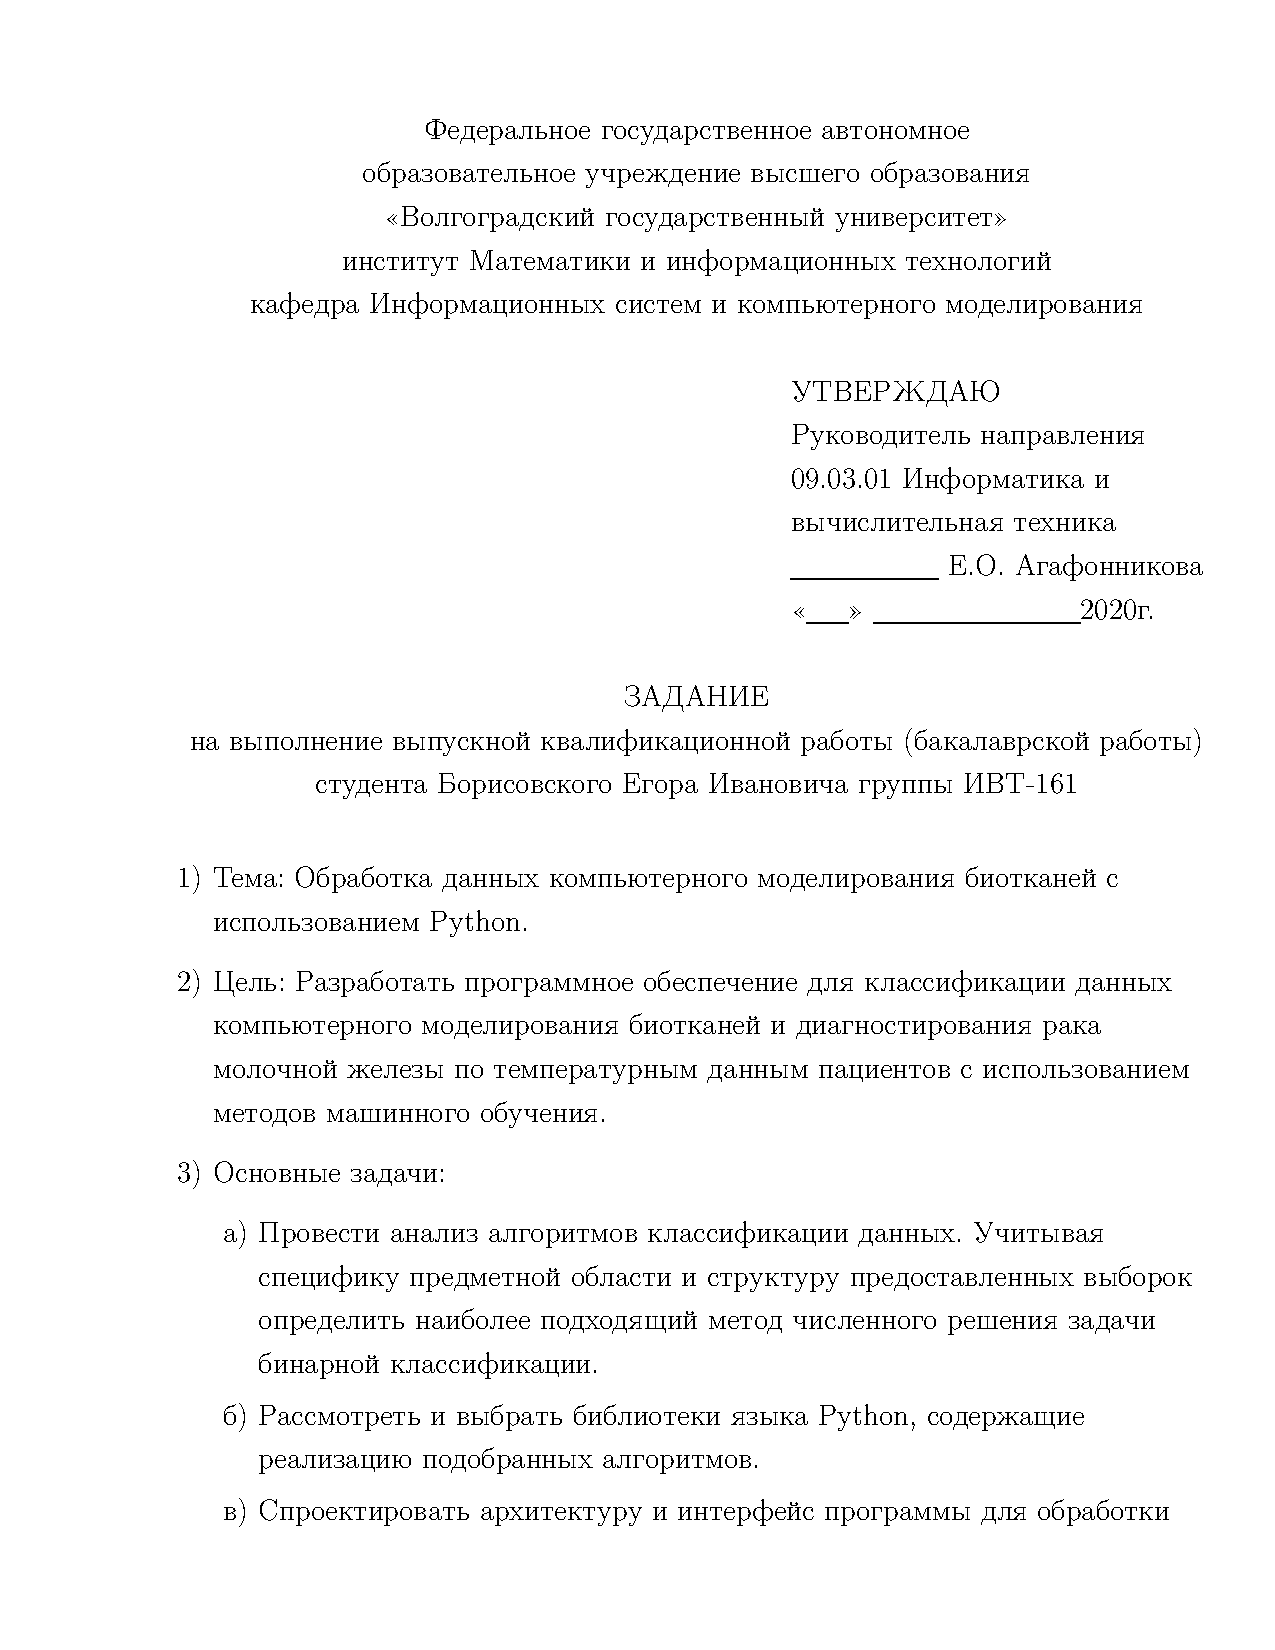
\includepdf[pages=-]{tz.pdf}

\end{document}